\documentclass[12pt,twoside]{article}
%\date{}   %uncommenting this erases the date
\usepackage{graphicx}
\usepackage{amsmath}
\usepackage{amssymb}
\usepackage{natbib}
\usepackage{verbatim}
\usepackage{floatpag}
\usepackage{subeqnarray}
\usepackage{mathrsfs}    %for special characters
\usepackage{cancel}  % to set terms in an equation to zero



\setlength{\textheight}     {9.0in}
\setlength{\textwidth}      {6.5in}
\setlength{\oddsidemargin}  {0.0in}
\setlength{\evensidemargin} {0.0in}
\setlength{\topmargin}      {0.0in}
\setlength{\headheight}     {0.0in}
\setlength{\headsep}        {0.0in}
\setlength{\hoffset}        {0.0in}
\setlength{\voffset}        {0.0in}
\setlength{\parindent}      {0.0in}      %starting new line at extreme left

\graphicspath{{Figures/}}

\newcommand{\astrut}{\usebox{\astrutbox}}

\newcommand\GaPQ{\ensuremath{G_a(P,Q)}}
\newcommand\GsPQ{\ensuremath{G_s(P,Q)}}
\newcommand\p{\ensuremath{\partial}}
\newcommand\tti{\ensuremath{\rightarrow\infty}}
\newcommand\kgd{\ensuremath{k\gamma d}}
\newcommand\shalf{\ensuremath{{\scriptstyle\frac{1}{2}}}}
\newcommand\sh{\ensuremath{^{\shalf}}}
\newcommand\smh{\ensuremath{^{-\shalf}}}
\newcommand\squart{\ensuremath{{\textstyle\frac{1}{4}}}}
\newcommand\thalf{\ensuremath{{\textstyle\frac{1}{2}}}}
\newcommand\Gat{\ensuremath{\widetilde{G_a}}}
\newcommand\ttz{\ensuremath{\rightarrow 0}}
\newcommand\ndq{\ensuremath{\frac{\mbox{$\partial$}}{\mbox{$\partial$} n_q}}}
\newcommand\sumjm{\ensuremath{\sum_{j=1}^{M}}}
\newcommand\pvi{\ensuremath{\int_0^{\infty}%
  \mskip \ifCUPmtlplainloaded -30mu\else -33mu\fi -\quad}}

\newcommand\etal{\mbox{\textit{et al.}}}
\newcommand\etc{etc.\ }
\newcommand\eg{e.g.\ }



\newcommand{\bs}  [1]{\boldsymbol{#1}}
\newcommand{\del} {\nabla}
\newcommand{\bsh}  [1]{\boldsymbol{\hat{#1}}}
\newcommand{\ul}  {\underline}
\newcommand{\ol}  {\overline}
\newcommand{\pp} [2]{\frac{\p{#1}}{\p{#2}}}
\newcommand{\dd} [2]{\frac{d{#1}}{d{#2}}}
\newcommand{\lam}  [1]{{#1}^{\tiny{\lambda}}}
\newcommand{\conj} [1]{{#1}^*}
\newcommand{\mods} [1]{ \vert {#1} \vert ^2}

\newcommand{\ph} [1]{ \langle #1 \rangle }  % For phase shorthand

\newcommand{\bsp} [1]{ \bs { #1^{\perp} }  }  % For phase shorthand

\newcommand{\w} [1]{  { {#1}_{\scriptscriptstyle W} }  }  % For wave shorthand

\newcommand{\g} [1]{  { {#1}_{\scriptscriptstyle G} }  }  % For geostrophic shorthand

\newcommand{\io} [1]{  { {#1}_{\scriptscriptstyle {IO} } }  }  % For io shorthand

\newcommand{\iw} [1]{  { {#1}_{\scriptscriptstyle {IW} } }  }  % For io shorthand

\newcommand{\spc}[1] {\mathscr {#1} }

%%% short hands for two waves and geostrophic modes %%%

\newcommand{\wf} [1]{  { {#1}_{\scriptscriptstyle {W1} } }  }  % For wave 1 shorthand

\newcommand{\wfc} [1]{  { {#1}^*_{\scriptscriptstyle {W1} } }  }  % For wave 1 c.c. shorthand

\newcommand{\ws} [1]{  { {#1}_{\scriptscriptstyle {W2} } }  }  % For wave 2 shorthand

\newcommand{\wsc} [1]{  { {#1}^*_{\scriptscriptstyle {W2} } }  }  % For wave 2 c.c. shorthand

\newcommand{\gf} [1]{  { {#1}_{\scriptscriptstyle {G1} } }  }  % For geostrophic 1 shorthand

\newcommand{\gfc} [1]{  { {#1}^*_{\scriptscriptstyle {G1} } }  }  % For geostrophic 1 c.c shorthand

\newcommand{\gfsq} [1]{  { {#1}^2_{\scriptscriptstyle {G1} } }  }  % For geostrophic 1 squared shorthand

\newcommand{\gs} [1]{  { {#1}_{\scriptscriptstyle {G2} } }  }  % For geostrophic 2 shorthand

\newcommand{\gsc} [1]{  { {#1}^*_{\scriptscriptstyle {G2} } }  }  % For geostrophic 2 c.c shorthand

\newcommand{\gssq} [1]{  { {#1}^2_{\scriptscriptstyle {G2} } }  }  % For geostrophic 2 squared shorthand

%%% short hands for two waves and geostrophic modes %%%


\title{Two layer Shallow water system}

\author{Raghav}

\begin{document}

\maketitle

\section*{Two Layer RSW}



\begin{figure*}
\centering
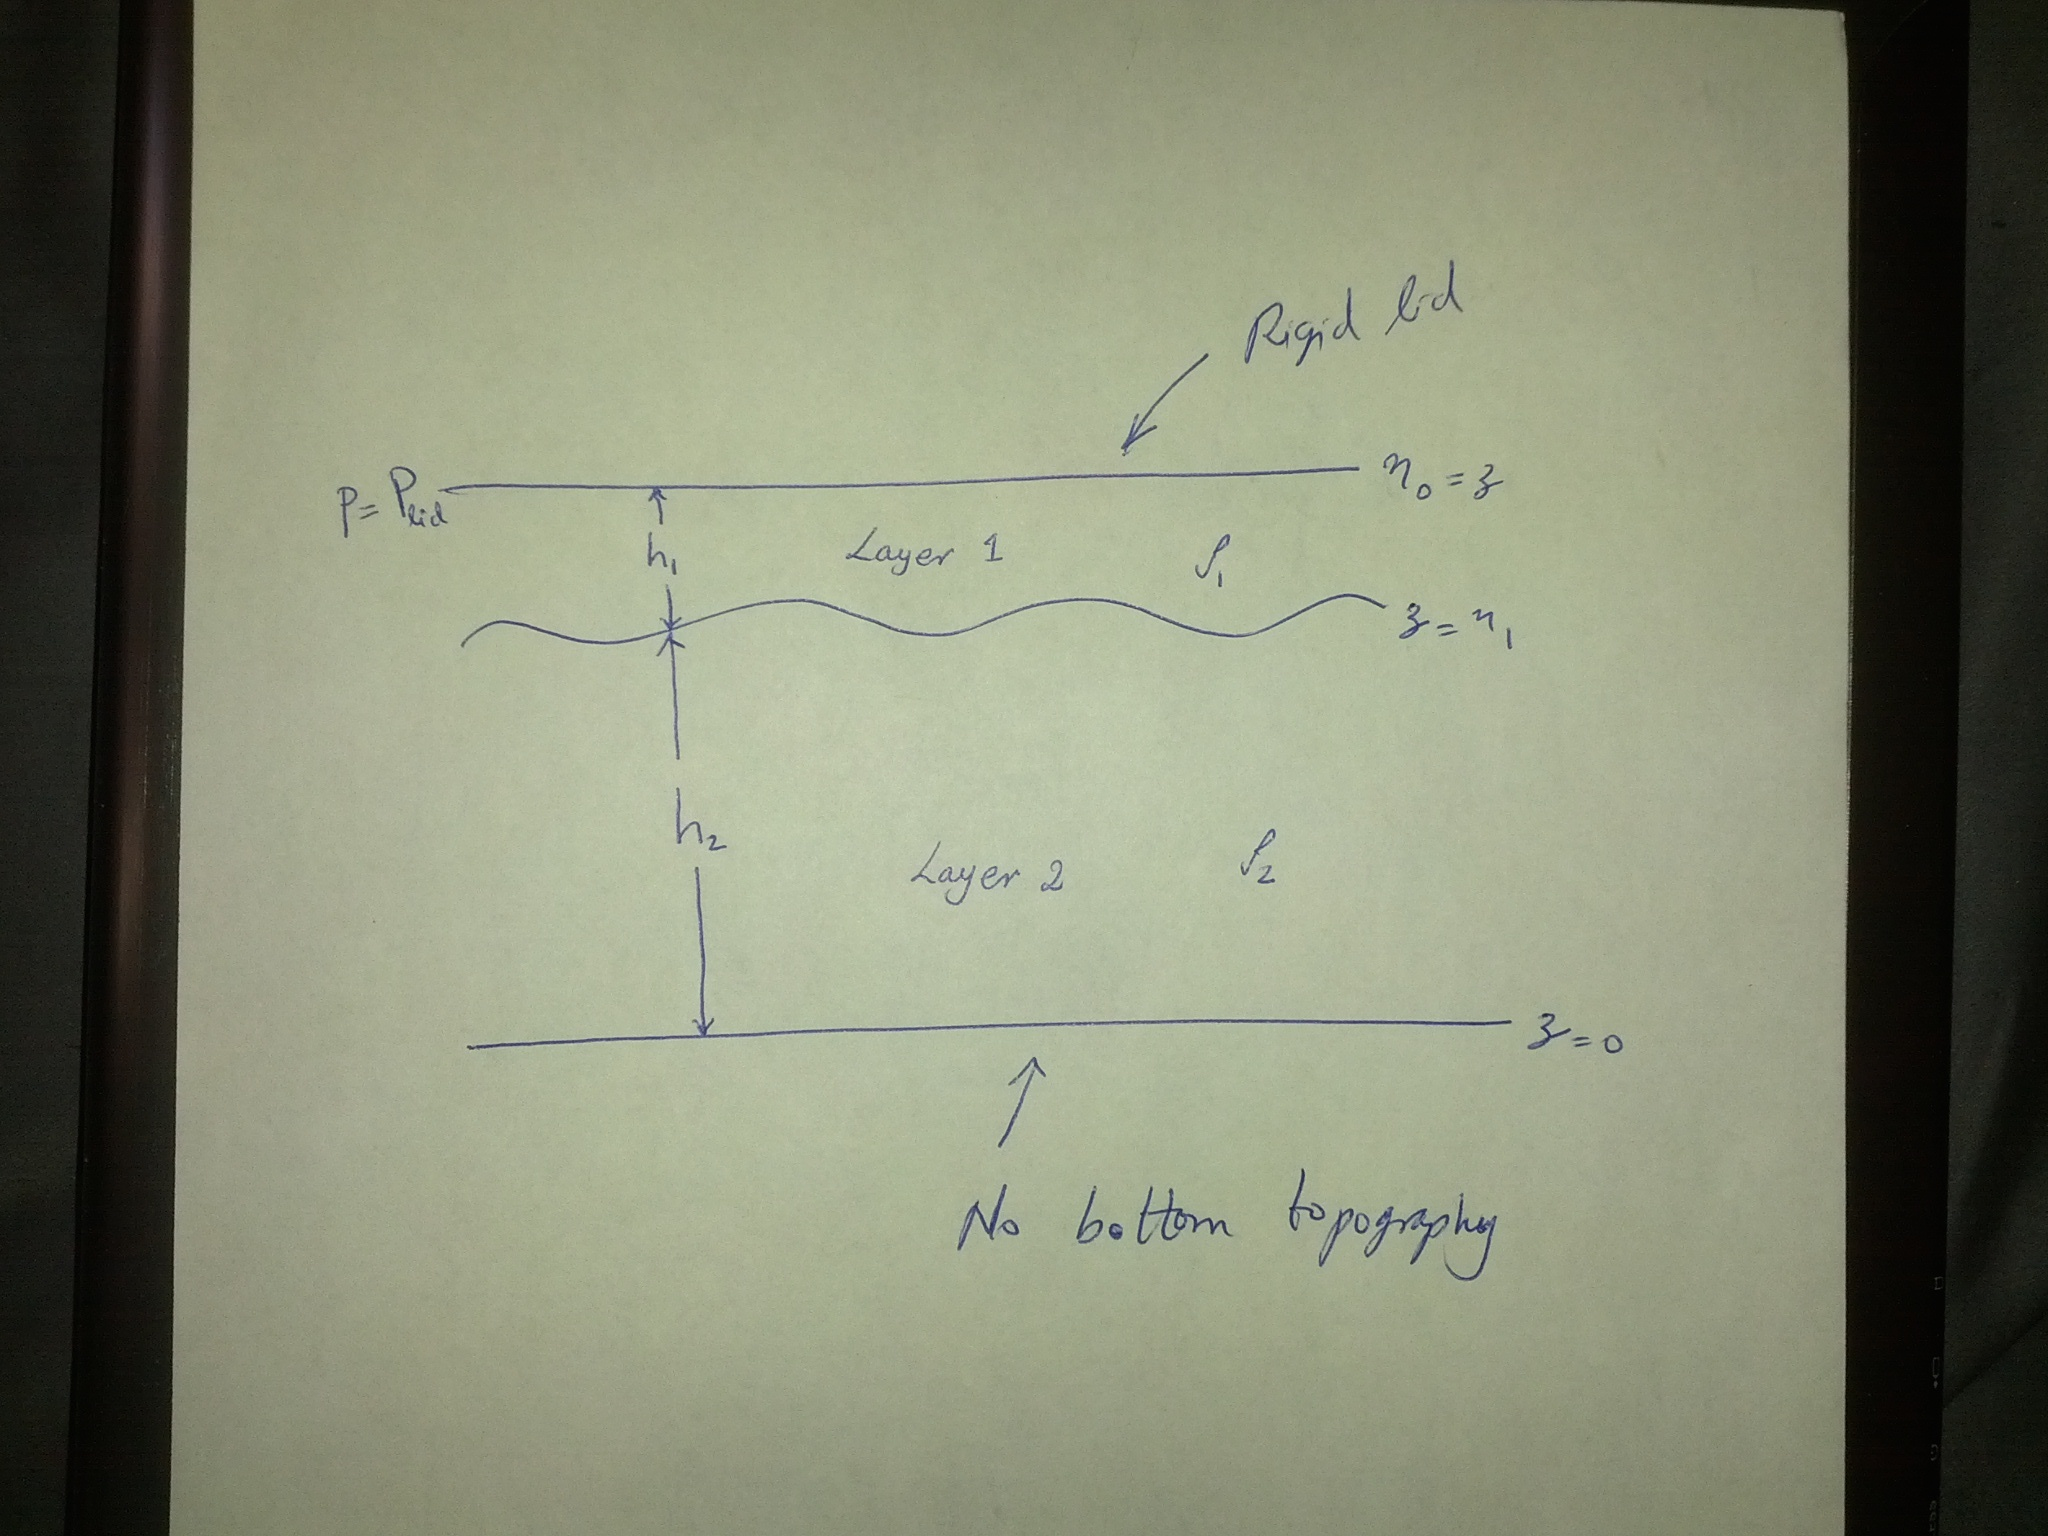
\includegraphics[width=5in,height=4in]{2_layer_sw.jpg}
\caption{Two layer shallow fluid system with no bottom topography and rigid lid.}
\label{sw2}
\end{figure*}

Consider the set up shown in the figure 1 consisting of a two layer  shallow fluid system with no bottom topography and rigid lid at top. The momentum equation in both the layers is given by
\begin{subequations}
\label{mom}
\begin{align}
\frac{D_1 }{D t} \bs v_1 + \bs f \times \bs v_1 = -\frac{1}{\rho _1} \del p_1  \\
\frac{D_2 }{D t} \bs v_2 + \bs f \times \bs v_2 = -\frac{1}{\rho _2} \del p_2
\end{align}
\end{subequations}
where the subscripts refer to the respective layers, e.g. $\bs v_1$ refers to velocity in layer 1 and $\frac{D_1 }{D t} = \pp{}{t} + \bs v_1 \cdot \del$.

Now, pressure in the respective layers are given by
\begin{subequations}
\begin{align}
&p_1 = p_{lid} + \rho _1 g (\eta _0 -z) \\
&p_2 = p_{lid} + \rho _1 g (\eta _0 -\eta _1) + \rho _2 g (\eta _1 -z)
\end{align}
\end{subequations}
where $p_{lid}$ is the lid pressure and $\eta _0$ is a constant due to rigid lid approx.
Substituition in \eqref{mom} gives
\begin{subequations}
\label{mom1}
\begin{align}
&\frac{D_1 }{D t} \bs v_1 + \bs f \times \bs v_1 = -\frac{1}{\rho _1} \del p_{lid}  \\
&\frac{D_2 }{D t} \bs v_2 + \bs f \times \bs v_2 = -\frac{1}{\rho _2}  ( \del p_{lid} + (\rho _2 - \rho_1)g \del \eta_1 )
\end{align}
\end{subequations}
If we demand that the bottom layer is at rest $\bs v_2 = 0$, then we obtain an expression for the lid pressure
\begin{equation}
\label{lid}
\del p_{lid} = - (\rho _2 - \rho_1)g \del \eta_1
\end{equation}
Substituition in the layer 1 equation gives 
\begin{equation}
\frac{D_1 }{D t} \bs v_1 + \bs f \times \bs v_1 = \frac{(\rho _2 - \rho_1)g}{\rho _1} \del \eta_1
\end{equation}
But height of the first layer, $h_1 = \eta _0 - \eta _1$. Therefore
\begin{equation}
\frac{D_1 }{D t} \bs v_1 + \bs f \times \bs v_1 = - \frac{(\rho _2 - \rho_1)g}{\rho _1} \del h_1 = - g' \del h_1
\end{equation}
which is the equation for layer 1. Also, by mass conservation,
\begin{equation}
\frac{D_1 }{D t} h_1 + h_1 \del \cdot \bs v_1 = 0
\end{equation}



% \bibliography{wv}


\end{document}


